\documentclass[a4paper, 12pt]{article}
%\usepackage[a4paper]{geometry}  % More space on A4 paper
\usepackage[a4paper, left=2cm, right=2cm, top=2cm, bottom=2cm]{geometry}
\usepackage{graphicx,epstopdf}
\usepackage{dcolumn}
\newcolumntype{d}[1]{D{.}{.}{#1}}
\usepackage{float}
\usepackage{tabularx,ragged2e,booktabs,caption}
\usepackage{array}
\usepackage[svgnames]{xcolor}
\usepackage{enumitem}
\usepackage{tikz}
\usepackage[utf8]{inputenc}
\usepackage{forest}
\usepackage{eurosym}
%%%%%%%%%%% mathematics %%%%%%%%%%%%%%%%%%
\usepackage{amsmath,amsfonts,amssymb, amsthm}
\usepackage{mathtools}
\usepackage[noend]{algpseudocode}
\usepackage{algorithm}
\usepackage{titling}
\setlength{\droptitle}{-5em}
\theoremstyle{definition}
\newtheorem{definition}{Definition}[section]
\newtheorem{theorem}{Theorem}
\newcommand\numberthis{\addtocounter{equation}{1}\tag{\theequation}}

% Use the bibliography, with \citet{}, \citep{}
\usepackage{natbib}
\usepackage{hyperref}


%%%%%%%%%%%%%%%%%%%%%%%%%%%% START HERE %%%%%%%%%%%%%%%%%%%%%%%%%%%% 

\title{\Huge Group Assignment I\\[0.5em]\large Advanced Econometrics, academic year 2026--2027}
\author{\large Phuc Nguyen (2779150)\\\normalsize Email: t.t.p.nguyen2@student.vu.nl\\[0.3cm]
\large Next (xxxxxxx)\\\normalsize Email: @student.vu.nl\\[0.3cm]
\large Next (xxxxxxx)\\\normalsize Email: @student.vu.nl\\[0.3cm]
\large Next (xxxxxxx)\\\normalsize Email: @student.vu.nl}
\date{\today}



\begin{document}
\maketitle
\newpage


\section*{Question 1}

\section*{Question 2}

\begin{figure}[H]
    \centering
    
\includegraphics[width=0.9\textwidth]{fig2.1.png}
    \caption{News impact curves of the GARCH-M-L model ($\mu = \lambda = 0$, $\alpha = 0.4$, $\sigma^2_{{t-1}} = 1$)}
    \label{fig:fig2.1}
\end{figure}


\section*{Question 3}
\begin{table}[H]
    \centering
    \caption{Descriptive statistics of the daily holding period returns}
    \begin{tabular}{lrrrr}
        \toprule
        & PFE & JNJ & MRK & AAPL \\
        \midrule
        Number of observations & 3270 & 3270 & 3270 & 3270 \\
        Mean & 0.041 & 0.046 & 0.057 & 0.107 \\
        Median & 0.000 & 0.036 & 0.046 & 0.089 \\
        Standard deviation & 1.368 & 1.076 & 1.306 & 1.783 \\
        Minimum & -7.735 & -10.038 & -9.863 & -12.865 \\
        Maximum & 10.855 & 7.998 & 10.408 & 11.981 \\
        Skewness & 0.223 & -0.150 & 0.083 & -0.076 \\
        Excess kurtosis & 5.294 & 9.370 & 6.637 & 5.360 \\
        \bottomrule
    \end{tabular}
    \label{tab:descrp_stats}
\end{table}


\begin{figure}[H]
    \centering
    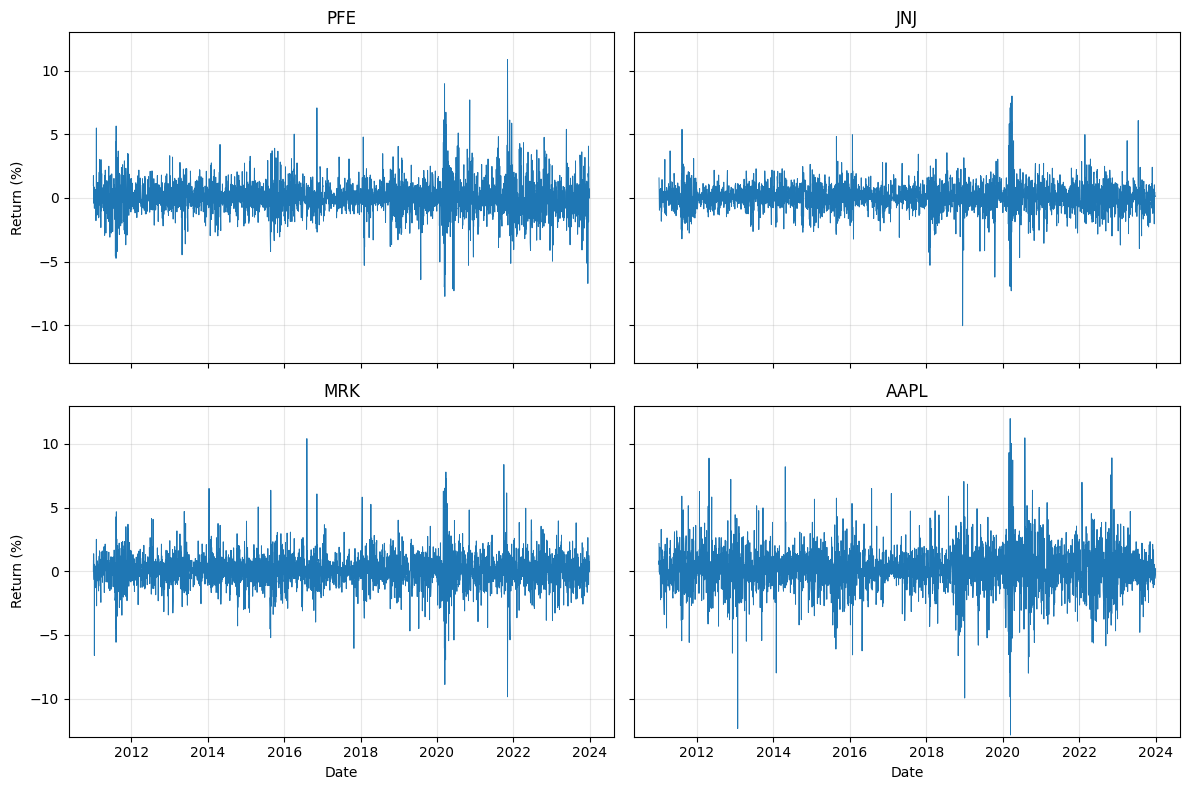
\includegraphics[width=0.9\textwidth]{fig3.1.png}
    \caption{Daily holding period returns of Pfizer, Johnson \& Johnson, Merck \& Co., and Apple.}
    \label{fig:fig3.1}
\end{figure}


\section*{Question 4}

\begin{table}[H]
    \centering
    \caption{Maximum likelihood estimates of the three volatility models}
    \label{tab:q4_estimates}
    \footnotesize
    \setlength{\tabcolsep}{3pt}
    \resizebox{\textwidth}{!}{%
    \begin{tabular}{l rrr rrr rrr rrr}
        \toprule
        & \multicolumn{3}{c}{PFE} & \multicolumn{3}{c}{JNJ} & \multicolumn{3}{c}{MRK} & \multicolumn{3}{c}{AAPL} \\
        \cmidrule(lr){2-4} \cmidrule(lr){5-7} \cmidrule(lr){8-10} \cmidrule(lr){11-13}
        & M1 & M2 & M3 & M1 & M2 & M3 & M1 & M2 & M3 & M1 & M2 & M3 \\
        \midrule
        $\mu$     & 0.037  & $-0.028$ & $-0.031$ & 0.072  & 0.058    & 0.033 & 0.066 & 0.077    & $-0.046$ & 0.154 & 0.072 & 0.108 \\
        $\lambda$ &        & 0.111    & 0.104    &        & 0.031    & 0.063 &       & $-0.015$ & 0.117    &       & 0.061 & 0.022 \\
        $\omega$  & $-0.027$ & $-0.028$ & $-0.025$ & $-0.002$ & $-0.002$ & 0.003 & 0.014 & 0.015 & 0.019 & 0.038 & 0.037 & 0.012 \\
        $\alpha$  & 0.036  & 0.036    & 0.043    & 0.025  & 0.025    & 0.026 & 0.039 & 0.040    & 0.040    & 0.090 & 0.089 & 0.073 \\
        $\beta$   & 0.961  & 0.963    & 0.953    & 0.923  & 0.924    & 0.916 & 0.906 & 0.904    & 0.906    & 0.874 & 0.875 & 0.915 \\
        $\delta$  &        &          & 0.029    &        &          & 0.017 &       &          & 0.039    &       &       & 0.071 \\
        $\gamma$  &        &          & 0.410    &        &          & 1.228 &       &          & 4.742    &       &       & 0.439 \\
        $\nu$     & 4.651  & 4.677    & 4.903    & 4.394  & 4.389    & 4.556 & 4.498 & 4.501    & 4.715    & 4.146 & 4.138 & 4.401 \\
        \midrule
        Log-lik & $-3769$ & $-3767$ & $-3753$ & $-3283$ & $-3283$ & $-3270$ & $-3893$ & $-3893$ & $-3868$ & $-4662$ & $-4662$ & $-4632$ \\
        AIC     & 7549    & 7546    & 7522    & 6576    & 6577    & 6557    & 7796    & 7798    & 7752    & 9335    & 9335    & 9280 \\
        BIC     & 7578    & 7581    & 7569    & 6605    & 6612    & 6603    & 7825    & 7833    & 7799    & 9364    & 9370    & 9327 \\
        \bottomrule
    \end{tabular}}

    \vspace{0.7em}
    \begin{minipage}{\textwidth}
        \footnotesize
        \textit{Notes:} M1, M2, and M3 are denoted as the GARCH, GARCH-M, and GARCH-M-L models, respectively.
    \end{minipage}
\end{table}

\section*{Question 5}


\section*{Question 6}




\end{document}